\chapter{Complex Langevin dynamics of spherical dimers}
\label{chapter:langevin_dynamics}
Much of the calibration theory discussed in Chapter 2 assumes that the target particle in question is a single sphere, one who's scattering and motion is easily computed. However, while working with dense colloidal suspensions, one often ends up trapping more than one sphere. Li and Arlt \cite{Li2008} studied the case of two microspheres trapped in a single OT and found that multiple trapped beads could be mistaken for a single trapped bead with altered trap stiffness. Theoretical studies on the case of two trapped microspheres by Xu~\textit{et~al.} \cite{Xu2005} employed a ray-optics based model to show that the two trapped beads are brought into physical contact with each other by optical forces and they also calculated the axial equilibrium positions of the two trapped beads as a function of their size. Experiments in \cite{Praveen2016} confirmed that the two trapped beads indeed experience different trap stiffnesses in the vicinity of the same potential well. There are further discussions looking into the dynamics of a whole host of asymmetrically shaped particles \cite{Loudet2014, ShengHua2005, Chetana2022}, their results all showing that predicting the behaviour an arbitrary shaped particle comes with great difficulty due to the fact that the optical force is dependent on a greater number of variables such as orientation and size factors.

In this chapter we consider how the addition of a second sphere into an optical trap can radically effect its dynamics, to the extent that one can no longer rely on typical calibration techniques to characterise the interactions.

%%%%%%%%%%%%%%%%%%%%%%%%%%%%%%%%%%%%%%%%%%%%%%%%%%%%%%%%%%%%%%%%%%%%%%%%%%%%%%%%
%%%%%%%%%%%%%%%%%%%%%%%%%%%%%%%%%%%%%%%%%%%%%%%%%%%%%%%%%%%%%%%%%%%%%%%%%%%%%%%%
\section{Positional and Orientational dependence of Trapping forces}

If we wanted to start from first principles and determine the trap strength on our target particle the first step would be to locate the harmonic traps relative to the trap focus. The methodology for computing optical forces has been covered extensively for a number of different trapping conditions \cite{RanhaNeves2019}, so it is relatively easy to compute the trapping force and determine where a simple sphere would be located relative to focal point of the laser. We can do so because the optical force is only dependent on the particle's relative position. If we instead consider a asymmetric dimer for example we see just by inverting the particle then a secondary harmonic trap can be found below the focus.

\begin{figure}[h!]
	\centering
	\begin{subfigure}{.475\linewidth}
		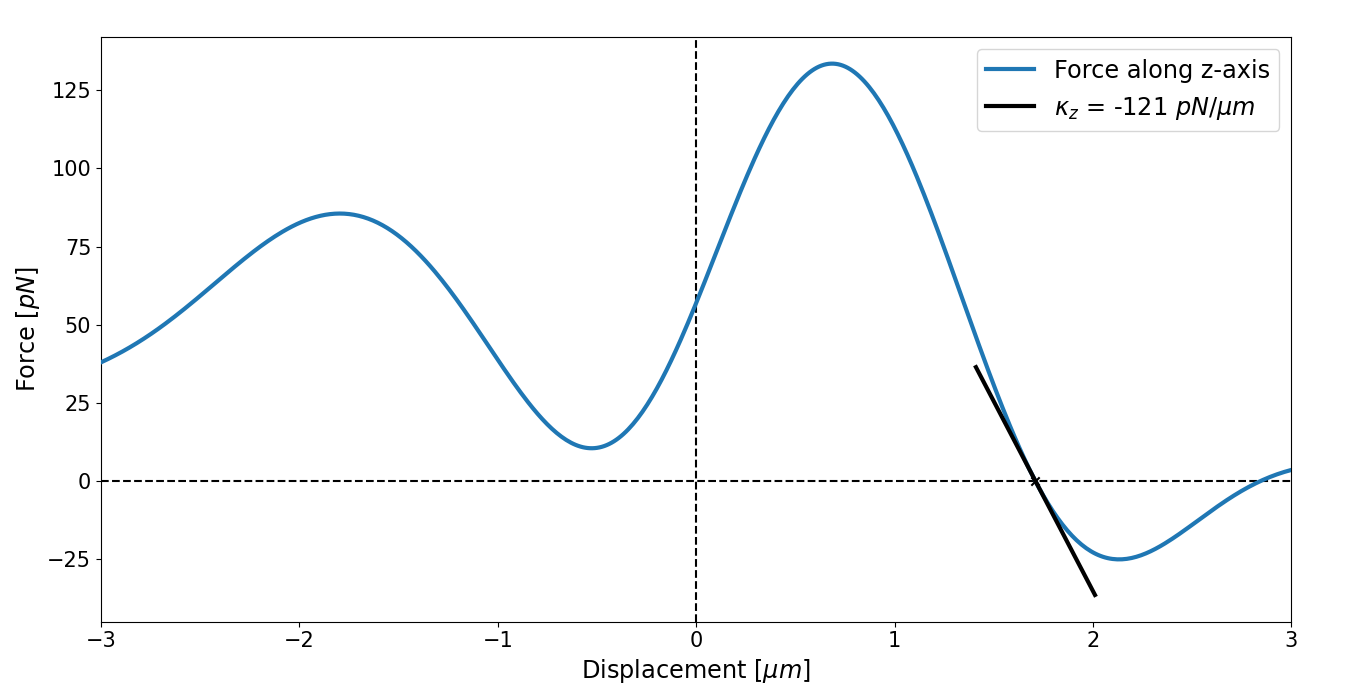
\includegraphics[width=\linewidth]{lam=2_theta=0.png}
		\caption{}
		\label{lam=2}
	\end{subfigure}\hfill % <-- "\hfill"
	\begin{subfigure}{.475\linewidth}
		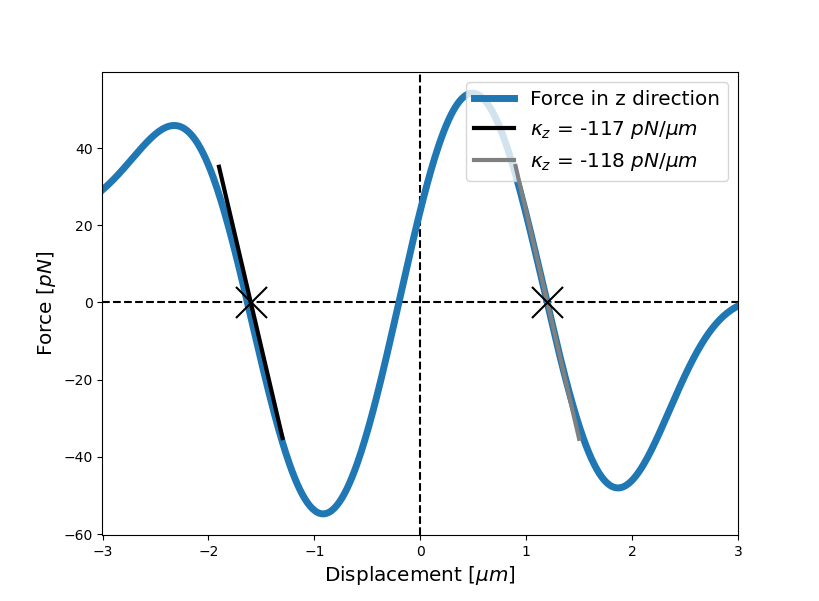
\includegraphics[width=\linewidth]{lam=2_theta=180.png}
		\caption{}
		\label{lam=2_inverted}
	\end{subfigure}\hfill % <-- "\hfill"
	\medskip
	\begin{subfigure}{.475\linewidth}
		\centering
		\raisebox{65pt}[0pt][0pt]{\makebox{}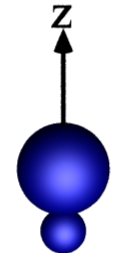
\includegraphics[width=0.3\linewidth, keepaspectratio]{theta=0.png}}
		\label{large over small}
	\end{subfigure}
	\begin{subfigure}{.475\linewidth}
		\centering
		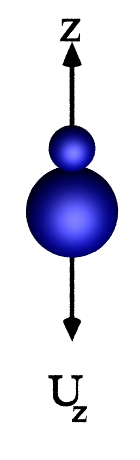
\includegraphics[width=0.3\linewidth, keepaspectratio]{theta=180.png}
		\label{small_over_large}
	\end{subfigure}
	\caption{Plots of force vs displacement of the point of the contact of the spheres (µm) for the case of a dimer of size ratio 2. (a) is the case where the smaller sphere is orientated with the beam propagation direction. (b) is the inverted case, smaller sphere oriented against the propagation direction. Renders to visualise the dimer orientation are shown below each plot The black lines on each force-curve is a linear fit with the slope being reported as the trap stiffness in the legend.}
\end{figure}

We can see that the trap below the focus is comparable in strength to above the focus, however the difference in the transverse strength is far more noticeable. As shown below in Fig~\ref{fig:transverse_force}, the dimer's orientation and relative position significantly changes the force curve; not only is the trap wider when inverted but the trap stiffness is increased. This highlights one of the challenges involved with studying asymmetric particles, even though its a simple enough process to trap them they maybe characterised very differently depending on their relative position and orientation towards the trap. This can have a significant impact on rheological studies - or attempting to probe any local property - as the variance in trap strength can result in large errors over repeated measurements. 
\begin{figure}[h!]
	\centering
	\label{fig:transverse_force}
	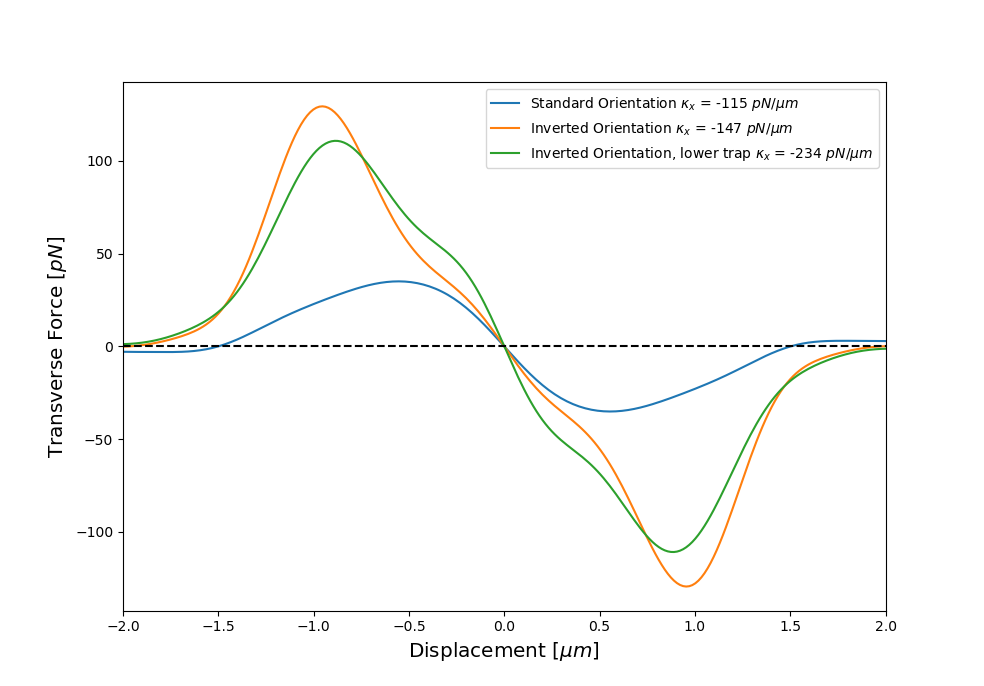
\includegraphics[width=0.67\linewidth]{transverse_force.png}
	\caption{Plots of force vs displacement of the point of the contact of the spheres (µm) for the case of a dimer of size ratio 2 while being displaced in the transverse plane. With the blue curve representing the force response for a dimer in its standard orientation, orange being the inverted case, and green the same case but placed below the focus.}
\end{figure}

For completeness the harmonic traps were located for dimers across a range of size ratios - from $a_1/a_2 = 1$ to $a_1/a_2=10$ - while also recording the trap stiffness for each trap. As $a_2$ decrease the dimer begins to approximate a single homogenous sphere - at least in terms of location and trap strength. However, for intermediate sized dimers (between $a_1/a_2 = 1.1$ to $a_1/a_2=4$), a second harmonic trap appeared below the trapping focus. Previous work using the ray-optics model have confirmed even in the case that two spheres begin separated the electric field will align the molecules as such that they make contact and are trapped together about a single trapping position \cite{Xu2005}. Furthermore it has been shown through proper manipulation of the Gaussian or Bessel beam modes that any number of trapping potentials can be developed \cite{Shahabadi2020}. This result however, is the first example of an orientation dependent trapping situation using only a $TEM_00$ beam. 

\begin{figure}[h!]
	\centering
	\begin{subfigure}{0.85\linewidth}
		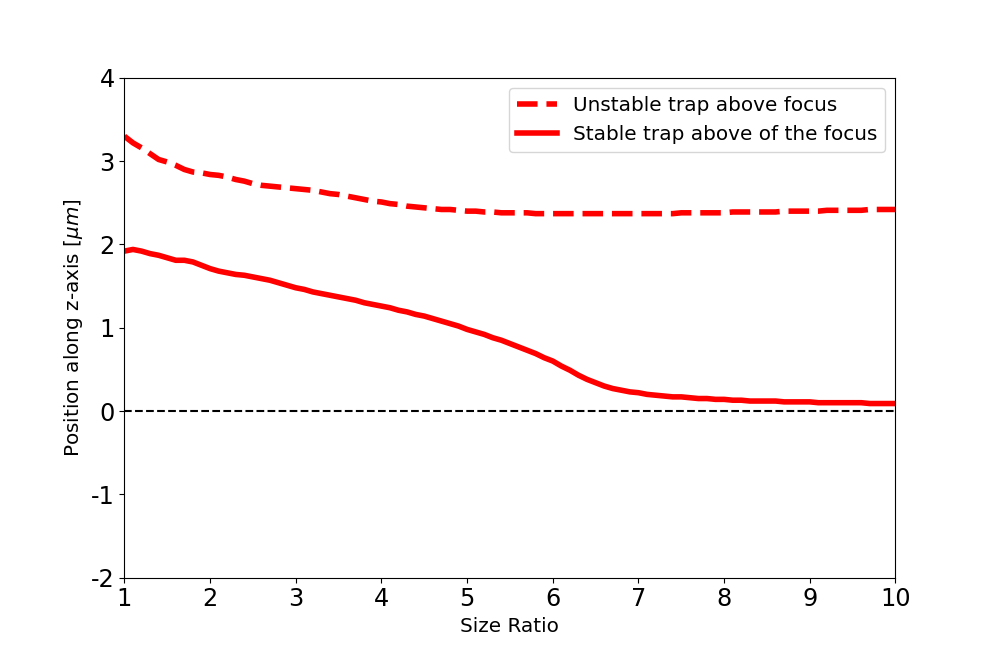
\includegraphics[width=\linewidth]{Equillibrium_positions.png}
		\caption{}
		\label{eq_pos}
	\end{subfigure}\hfill % <-- "\hfill"
	\medskip
	\begin{subfigure}{0.85\linewidth}
		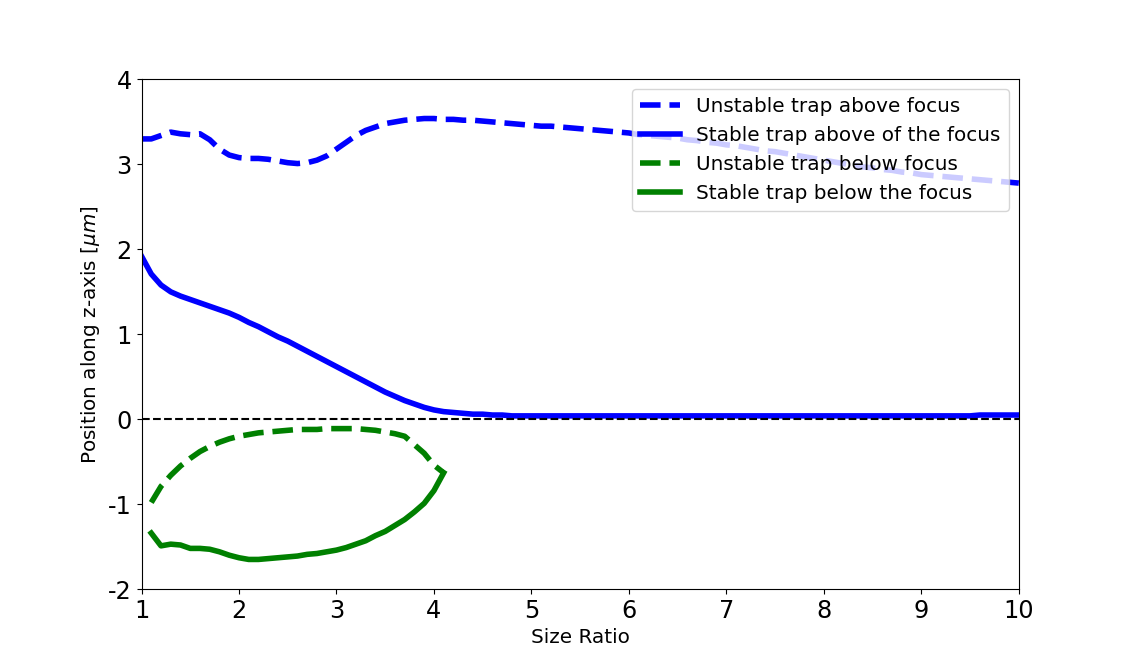
\includegraphics[width=\linewidth]{Equillibrium_positions_inverted.png}
		\caption{}
		\label{eq_pos_inverted}
	\end{subfigure}
	\caption{Equilibrium positions of optically trapped dimers with varying size ratio, dotted lines represent unstable traps whereas solid lines represent stable trapping positions. (a) shows that dimers with their smaller sphere orientated away from the focus have an expected single trapping position. (b) shows that when the same dimer is inverted $180^\circ$ there are now stable traps along the beam axis, one below the focus and one above the focus.}
\end{figure}
\newpage
\subsection{Non-trivial harmonic traps}\label{sec:off-axis}
Computing the equilibrium positions when a dimer is aligned with the electric field is relatively simple as the orientational torque is minimised (see Eq.\ref{eq:opt_torque}), meaning once trapped the dimer is unlikely to change orientation enough to escape the trap. However, that does not rule out the possibility that there is a stable orientation that is not strictly vertical, in fact most experimental work with symmetric dimers will trap them lying perpendicular to the beam direction \cite{Ahn2018}. Unlike before where we can simply find the trap by varying the dimer's vertical position its instead more prudent to run a multitude of smaller simulations at a variety of starting positions and orientations. An example for a dimer of size ratio 2 is shown below:
\begin{figure}[h!]
	\centering
	\begin{subfigure}{0.67\linewidth}
		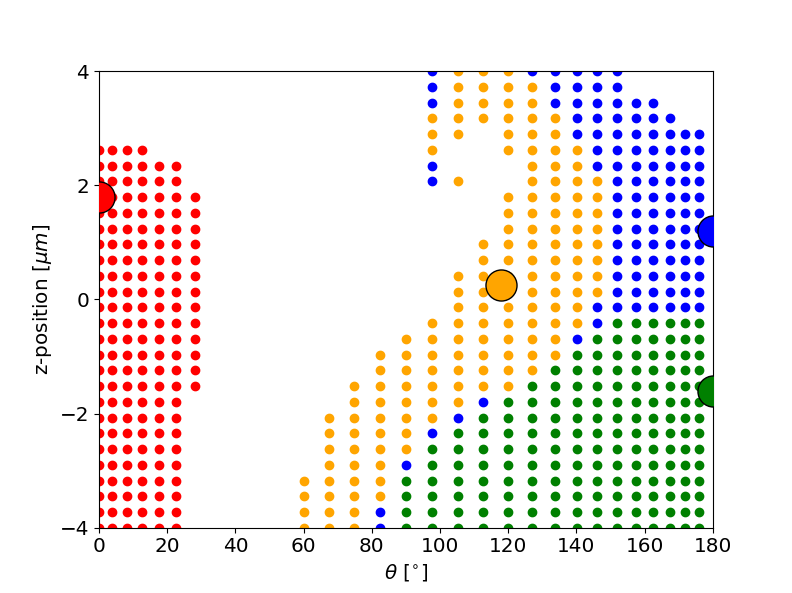
\includegraphics[width=\linewidth]{off_axis_trap.png}
		\caption{}
	\end{subfigure}
	\begin{subfigure}{0.32\linewidth}
		\raisebox{0pt}[0pt][0pt]{\makebox{}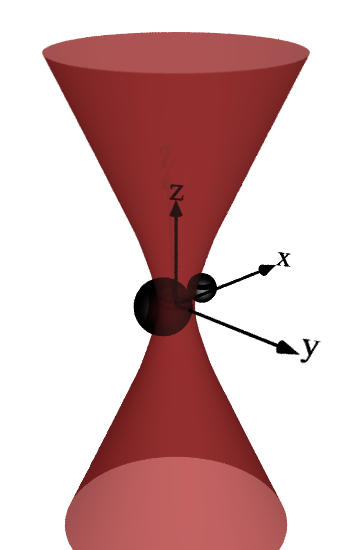
\includegraphics[width=\linewidth, keepaspectratio]{off_axis_render.png}}
		
		\caption{}
	\end{subfigure}
	\captionsetup{hangindent=2.35cm}
	\caption{Trajectory map of simulations ran using a dimer of size ratio 2 with a laser power of 500 mW. The stable points are indicated by the larger spheres and the starting conditions are colour coded to match the stable point they end up in. Right hand render shows a dimer in its off-axis configuration}
\end{figure}
Interestingly while the trap strength of these off-axis traps are 
similar in magnitude to the vertically aligned dimers, but when 
the laser power is lowered (around 5 mW) the traps become metastable 
resulting in the dimer escaping from after some random time while 
within the trap. If the overall potential depth could be characterised 
then dimers placed into this orientation could be used as a 
micro-scale temperature alarm, where by fine tuning of the dimer's 
parameters would allow you to construct a potential well that can 
only be escaped when the local fluid temperature exceeds a certain maximum value.  

%%%%%%%%%%%%%%%%%%%%%%%%%%%%%%%%%%%%%%%%%%%%%%%%%%%%%%%%%%%%%%%%%%%%%%%%%%%%%%%%
%%%%%%%%%%%%%%%%%%%%%%%%%%%%%%%%%%%%%%%%%%%%%%%%%%%%%%%%%%%%%%%%%%%%%%%%%%%%%%%%
\section{Continuous rotational motion due to second-order scattering}

One aspect that has yet to be covered in depth with regards to
spherical aggregates of any construction is their interaction with
circularly polarised light. Typically the spin density of an electric
field cannot be reduced in homogenous medium due to the fact that the
spin angular momentum is conserved locally. In which case the only way
to transfer angular momentum to use an object that is anisotropic.
This is seen most clearly with birefringent materials, due to fact that
the crystal lattice itself is anisotropic, a circularly polarised beam
will transfer an optical torque that is proportional to the difference in 
the refractive index of the particle. The optical torque is given as:
\begin{equation}
	\label{eq:opt_torque}
	\begin{aligned}
		\tau_{opt} = \frac{\epsilon}{2\omega_{laser}}E_0^2 (1-cos(kd(\Delta n))sin2\phi)
	\end{aligned}
\end{equation}
Where $\Delta n$ is the difference in refracive indices of the 
particle, and $\phi$ indicates the phase shift in the electric field
(for circular polarised light $\phi= \pi/4$) However, theoretical and
experimental work by \cite{Yevick2017} found that highly focused
Gaussian beams could produce second order effects in the Rayleigh
regime resulting in a photo-kinetic force that results in orbital
motion about the beam's central axis. This effect is rather minimal
for single sphere's, resulting in a orbital frequency on the order of
$10^{-1}\,{\rm Hz}$, with an order of magnitude difference when
trapping aggregates of spheres.  They computed the circulation rate by
computing the time-average probability flux; however, when extended to
the Mie regime we see a completely different behaviour, instead
experiencing an optical torque about their long axis.S This rotation
was first noted by Vigilante and co-workers who only considered this
behaviour for a symmetric dimer \cite{Vigilante2020}; we run number of
simulations for differently sized dimers in a circularly polarised
trap and looked at the rotation rate.  We found that not only is the
rotation rate dependent on the size of the dimer, but also on its
orientation and therefore their axial position.

\begin{figure}[h]
  \centering
  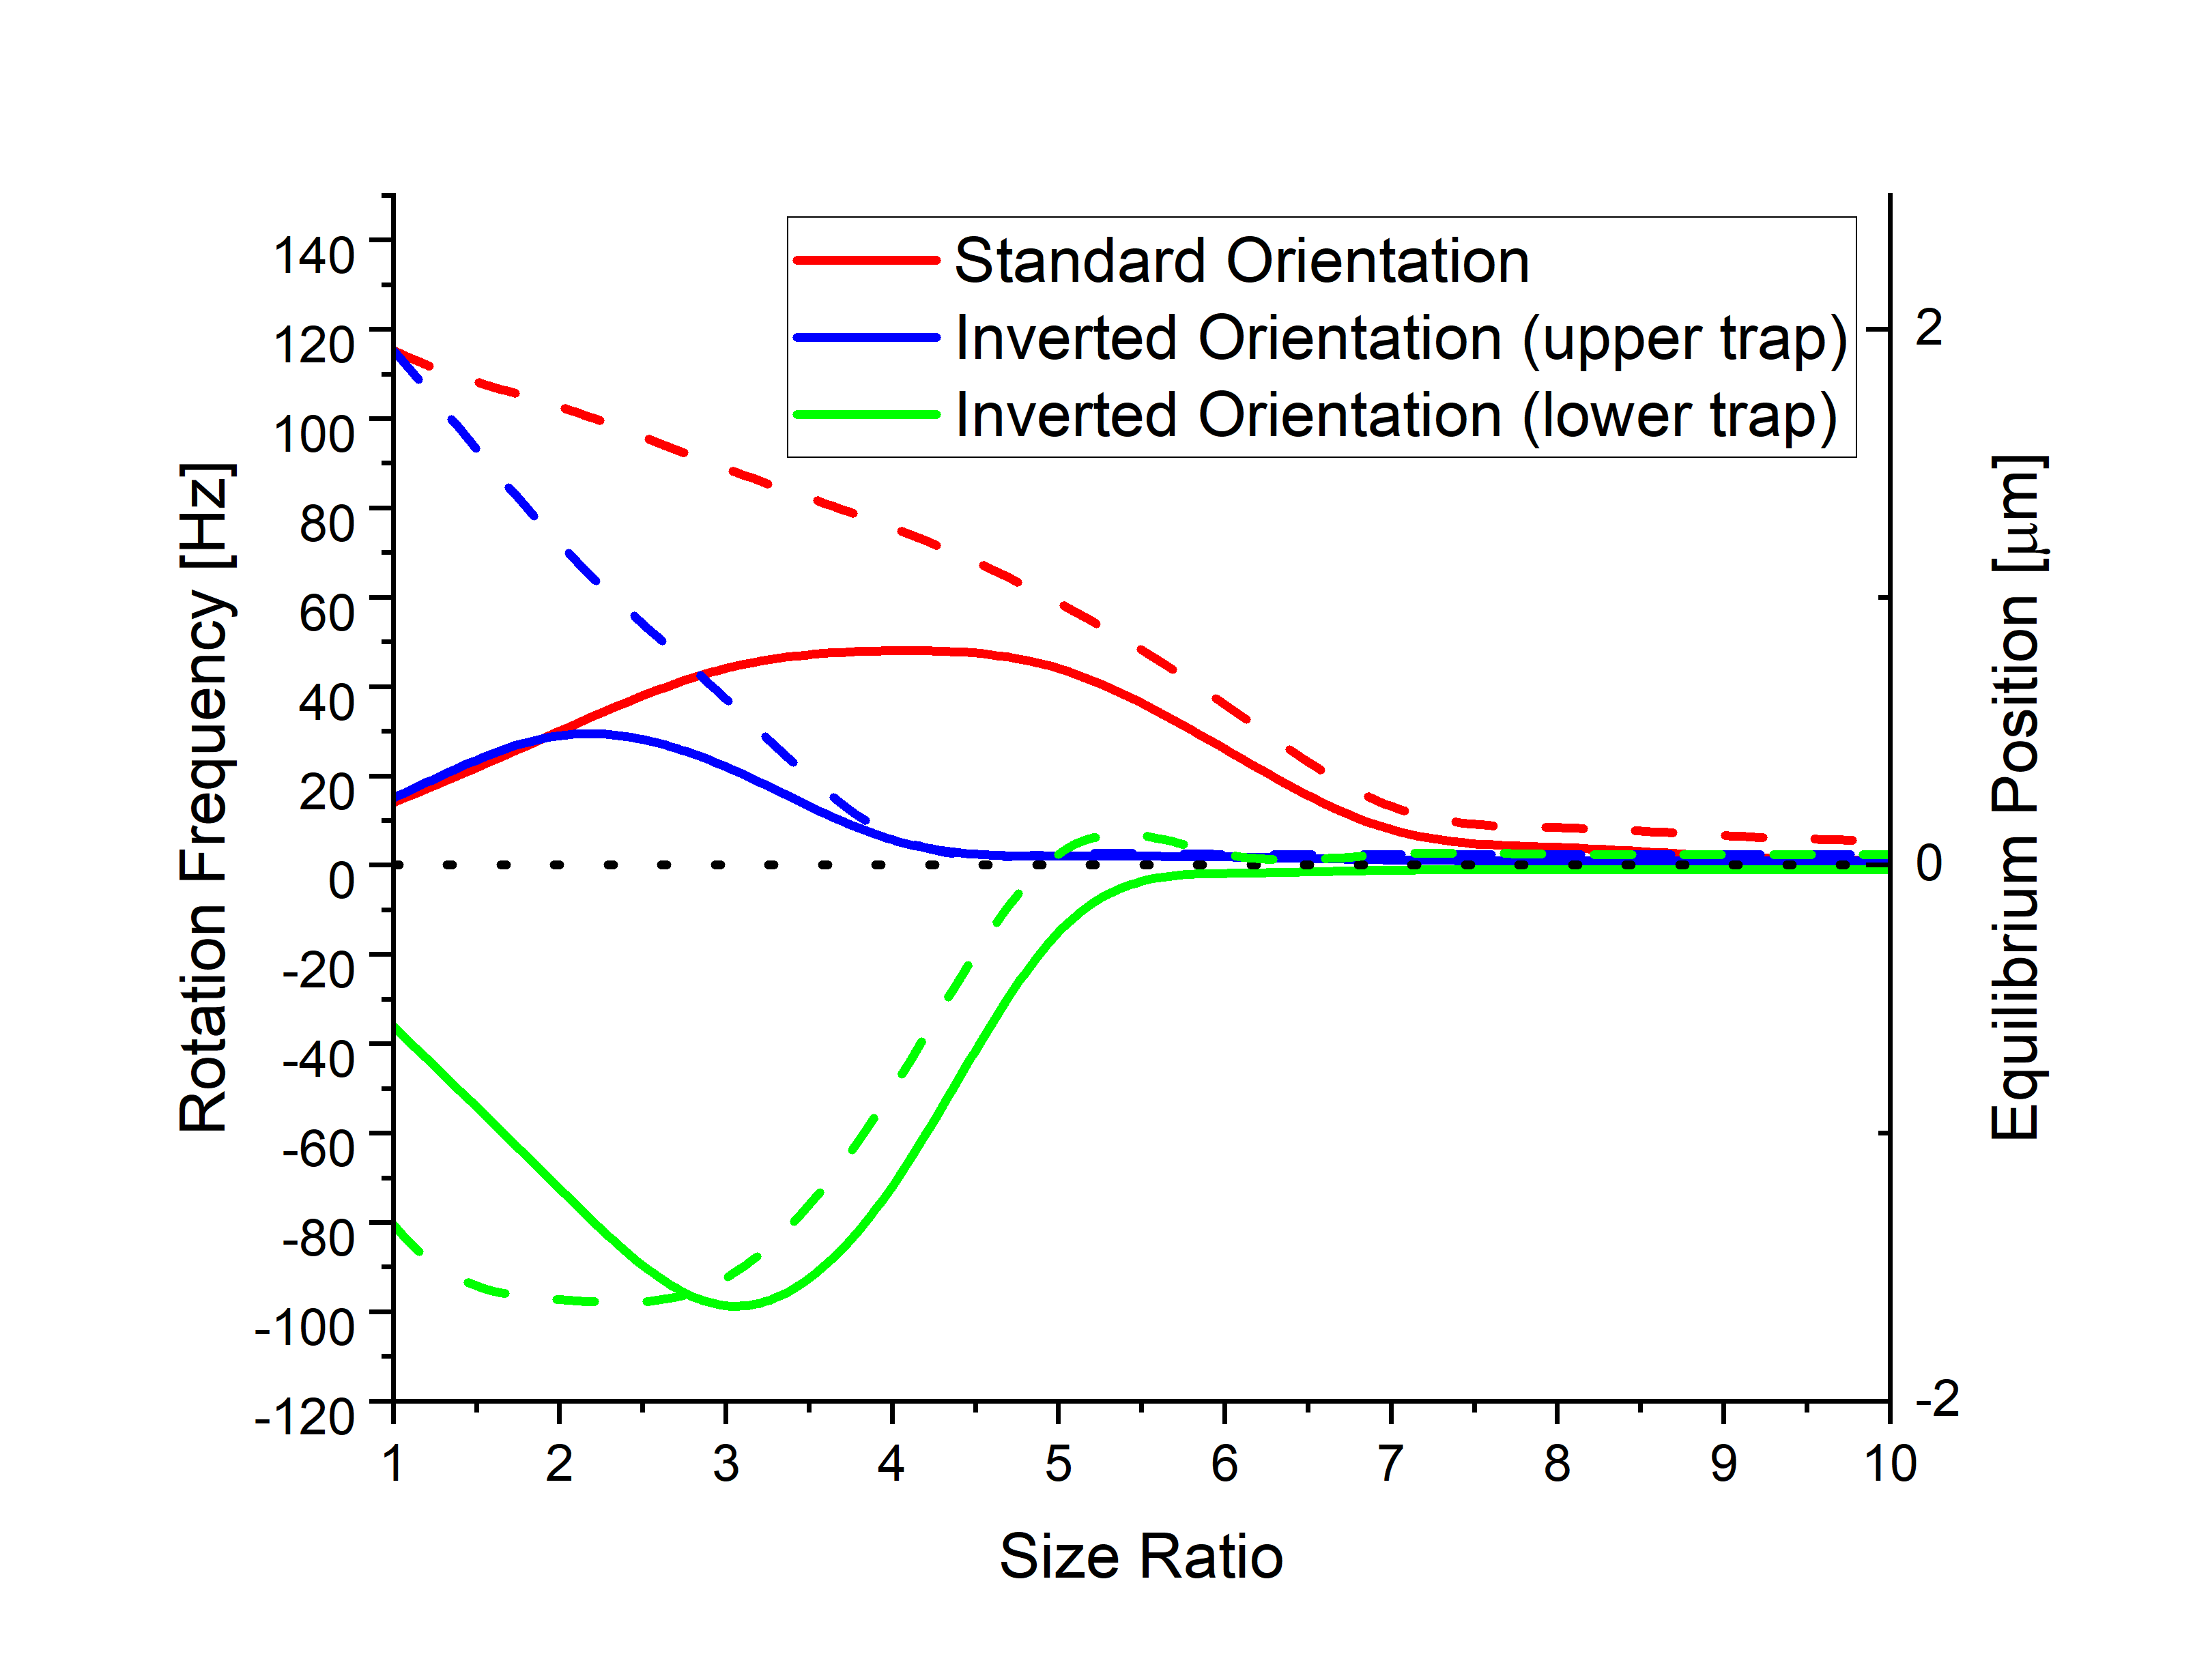
\includegraphics[width=0.65\linewidth]{rotation_rate_vs_size.png}
  \caption{Rotation rate plotted against dimer size ratio for a variety of different simulation scenarios. The red line is for the case where the larger sphere is above the smaller sphere. The blue line is the inverted case, while the initial position is above the focus of the trap. And lastly the green line is again for the inverted case, but when the dimer's initial position is below the focus of the trap.}
\end{figure}

It is difficult to see from the graph, but the rotation rate never
truly goes down to zero, reaching a minimum of $2\,{\rm Hz}$, which would
imply that a second sphere of radius $200\,{\rm nm}$ is enough to
induce rotational motion.  We used MSTM to look at the stokes
parameters from the scattered field from a simple plane wave incident
on our dimer, the proportion of circularly polarised light is minimal
compared to the proportion of plane polarised light, which indicates
that this rotational motion is not due to any inhomogeneity in the
dimer that might impart angular momentum to the scattered beam - as
compared to a anisotropic scatterer like Vaterite.

These results are somewhat contrary to other work with silica dimers
\cite{Ahn2018, Debuysschere2023,Reimann2018}; previous experiments
have trapped the dimer in an orientation perpendicular to the beam
propagation direction.  The rotational motion is induced due to the
asymmetric geometry creating an unbalanced polarisation susceptibility
along its long axis as compared to its short axis; therefore its long
axis is aligned with the polarisation vector and can rotate
freely\cite{Ahn2018}.  This however cannot be the case with our
simulations as the dimer rotates about its long axis, meaning there
cannot be an asymmetric axis to align with the beam's polarisation
vector. Furthermore, we see a non-linear increase in the rotational
speed of our dimers with size, the drag torque from the surrounding
fluid is $\propto r^3$ so the expectation is that the rotation
frequency should fall off with increasing size.  This indicates that
the rotational motion is due to the shape asymmetry of the dimer and
not solely due to the beam's angular momentum.  Measurement of this
photo-kinetic force is difficult to achieve due to the fact that
previous analysis was conducted in the Rayleigh regime, where the
polarizability of our dimer can be approximated as:
\begin{align}
  \bold{p}({\bf r},t)
  =
  \alpha_x E_x({\bf r},t)\hat{\bf e}_x
  + \alpha_yE_y({\bf r},t)\hat{\bf e}_y
  + \alpha_zE_z({\bf r},t)\hat{\bf e}_z
\end{align}
where the polarizability is given as a 3D vector for the three
principle Cartesian directions.  In order to measure the magnitude of
second order contributions we would need to construct a dipole array
that fully captures the scattering of a dimer. Measuring the optical torque 
makes it clear that the polarizability is a contributing factor to this optical 
rotation phenomena. Rotating a symmetric dimer in the $x-z$ plane reveals 
that while the dimer can be rotated in an orientation perpendicular 
to the beam rotational torque is maximised when rotated while aligned with 
the optical axis.
\begin{SCfigure}
	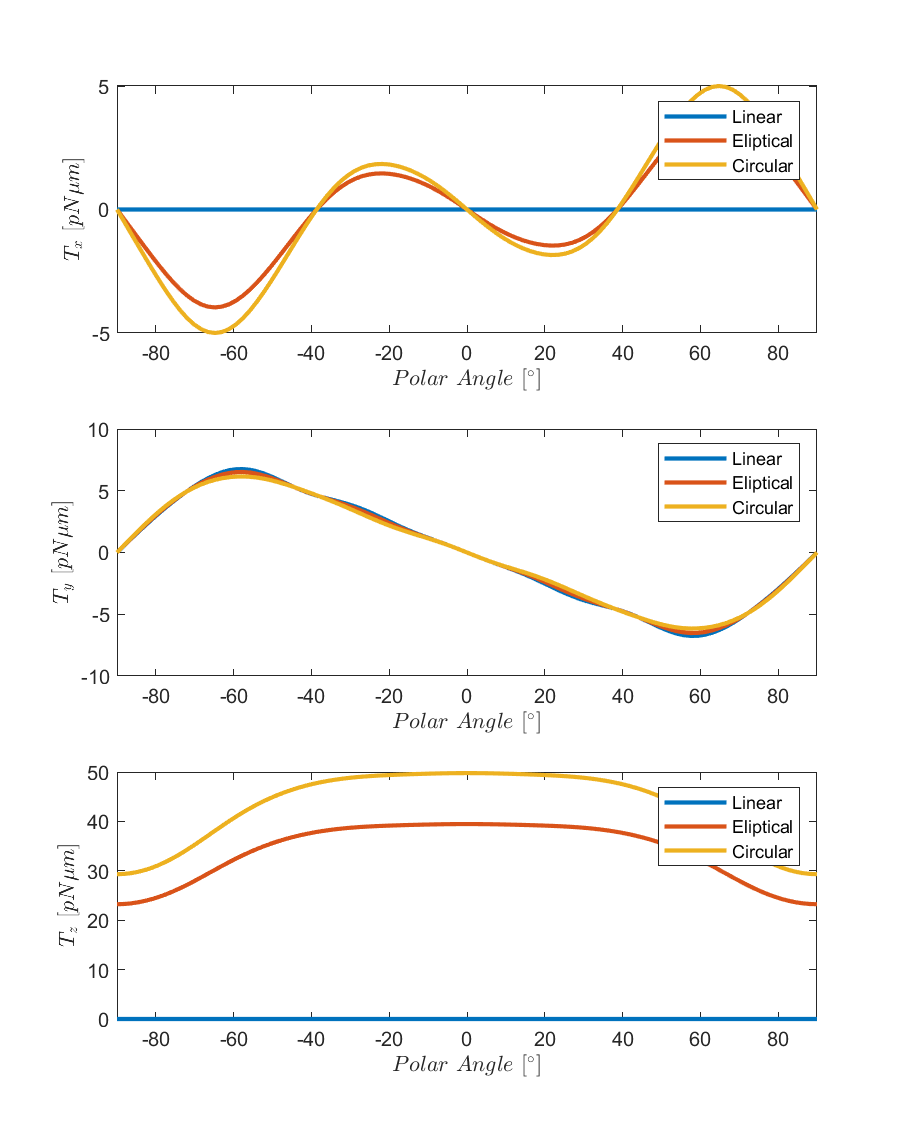
\includegraphics[width=0.7\linewidth,height= 22cm]{torque_different_polarisations.png}
	\caption{Optical torque against polar angle $\theta$ about the three primary axis (top: torque about the x-axis; middle: torque about the y-axis; bottom: torque about the z-axis) on a symmetric dimer in linear, elliptical, and circular polarisation beams. Diagram to the right is for visual clarity about the direction of $\theta$. \vspace{7.5cm}}
\end{SCfigure}
\newpage

\subsection{Gyroscopic Precession using asymmetric dimers}
As mentioned in section~\ref{sec:off-axis} for specificity sized dimers 
there is the potential for non-vertical trapping orientations in which 
the dimer is located in a harmonic trap. When trapped by a circularly 
polarised light these dimers exhibit gyroscopic precession, demonstrating 
rotational motion not just about its long axis, but also around the 
optical axis of the beam. This gyroscopic motion has been demonstrated 
previously in nanoparticles \cite{Zhu2021, Rashid2018, Hoang2016, Kuhn2016} 
but has not been observed for micron scale aggregates. Since the torque is 
computed by evaluating the beam coefficients it can be difficult to 
apply this result to micro-rheology experiments as one would need to know
the exact magnitude of the optical torque ahead of time in order to make
estimations about the local fluid viscosity. This is trivial for a birefringent
spherical particle, less so for spherical aggregates whose final position and 
orientation are unknown.

\comment{Need to add figure here demonstrating the rotational behaviour but not sure how to best convey that motion. Perhaps just a simple trajectory diagram showing the particles motion (position in the first column, $u_x$ in the second, then $u_y$, then $u_z$).}

\section{Characterisation of asymmetric dimers via PSD analysis}


%%%%%%%%%%%%%%%%%%%%%%%%%%%%%%%%%%%%%%%%%%%%%%%%%%%%%%%%%%%%%%%%%%%%%%%%%%%%%%%%
%%%%%%%%%%%%%%%%%%%%%%%%%%%%%%%%%%%%%%%%%%%%%%%%%%%%%%%%%%%%%%%%%%%%%%%%%%%%%%%%
\section{Conclusions}
